\documentclass{beamer}

\usepackage{polyglossia}
\usepackage{fontspec}
\usepackage{nameref}
\usepackage{ifthen}

\usefonttheme{professionalfonts}
\usetheme{Antibes}
\useoutertheme{infolines_foot}
\setbeamercovered{transparent=20}

\usepackage[math-style=ISO,vargreek-shape=unicode]{unicode-math}
\setdefaultlanguage[spelling=modern,babelshorthands=true]{russian}
\setotherlanguage{english}

\defaultfontfeatures{Ligatures={TeX}}
\setmainfont{CMU Serif}
\setsansfont{CMU Sans Serif}
\setmonofont{CMU Typewriter Text}
\setmathfont{Latin Modern Math}
\AtBeginDocument{\renewcommand{\setminus}{\mathbin{\backslash}}}

\makeatletter
\newcommand*{\currentname}{\@currentlabelname}
\makeatother
\def\t{\texttt}

\newcommand{\cimg}[2]{%
	\begin{center}%
		\ifthenelse{\equal{#2}{}}{%
			\includegraphics[width=0.75\linewidth]{#1}
		}{%
			\includegraphics[width=#2\linewidth]{#1}
		}%
	\end{center}%
}

\title[Граф связей между контигами]{Построение графа связей геномных последовательностей}
\author[Черникова Ольга]{Черникова Ольга\\
	Руководитель: Пржибельский Андрей Дмитриевич}
\institute{СПб АУ РАН}
\date{Осень 2016}

\begin{document}

\begin{frame}
	\titlepage
\end{frame}

\section{Постановка задачи}

\begin{frame}[t]{Постановка задачи}
	\begin{itemize}
		\item Хочется собрать ДНК:
		\cimg{p1_1.png}{1}
		\item Реально получается собрать только какие-то его части(контиги):
		\cimg{p1_2.png}{0.25}
		\item \textbf{Цель проекта} "--- востновить порядок следования контигов:
		\cimg{p1_3.png}{1} 
	\end{itemize}
\end{frame}

\begin{frame}[t]{Задачи}
\begin{itemize}
\item Иследовать возможные варианты построения графа по ридам РНК. 
\item Объединить разные виды связей между контигами в один граф. 
\item Решить проблему с подбором параметров для фильтрации графа. 
%\item Создать программный продукт для построения 
%графа связей между контигами.  
\end{itemize}
\end{frame}	

\section{Методы решения}
\subsection{Архитектура}
\begin{frame}[t]{Архитектура}
Задача делится на две части:
\begin{itemize}
\item Построение графа связей
\item Фильтрация
\end{itemize}	
\cimg{src.jpg}{0.65}
\end{frame}
\subsection{Построение графа}
\begin{frame}[t]{Построение графа}
\cimg{BuilderClassDiagram.jpg}{1}	
\end{frame}
\begin{frame}[t]{Способы поcтроения}
\begin{itemize}
	\item по парным ридам ДНК
	\item по парным ридам РНК
	\item по ридам РНК на стыке экзонов
	\item по эталонной сборке
\end{itemize}
\cimg{p5.png}{1.21}
\end{frame}

\subsection{Фильтрация графа}
\begin{frame}[t]{Фильтрация графа}
	\begin{itemize}
		\item Консольное приложение для фильтрации и отображения графа.
		\item Десериализует граф. 
		\item В зависимости от введеных команд фильтрует граф. 
		\item Декомпозирует граф для удобства вывода.
		\item Выводит граф в dot формате одним из способов в зависимости от команды. 
	\end{itemize}
\end{frame}

\section{Результаты}
\begin{frame}[t]{Результаты}
	\begin{itemize}
		\item Программа для нахождения связей
		между контигами различными способами. 
		\item Программа с различными возможностями для 
		визуализации и фильтрации получившегося графа. 
		\item Удалось улучшить сборку С.elegans.
		\begin{center}
		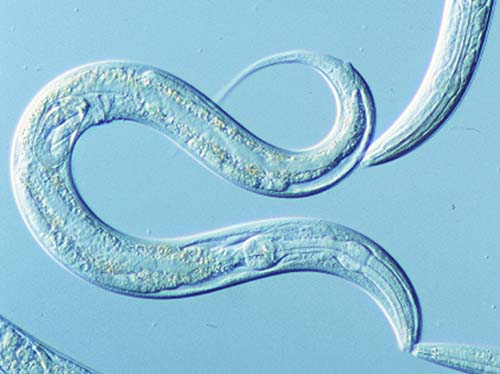
\includegraphics[width=0.35\linewidth]{celegans.jpg}
		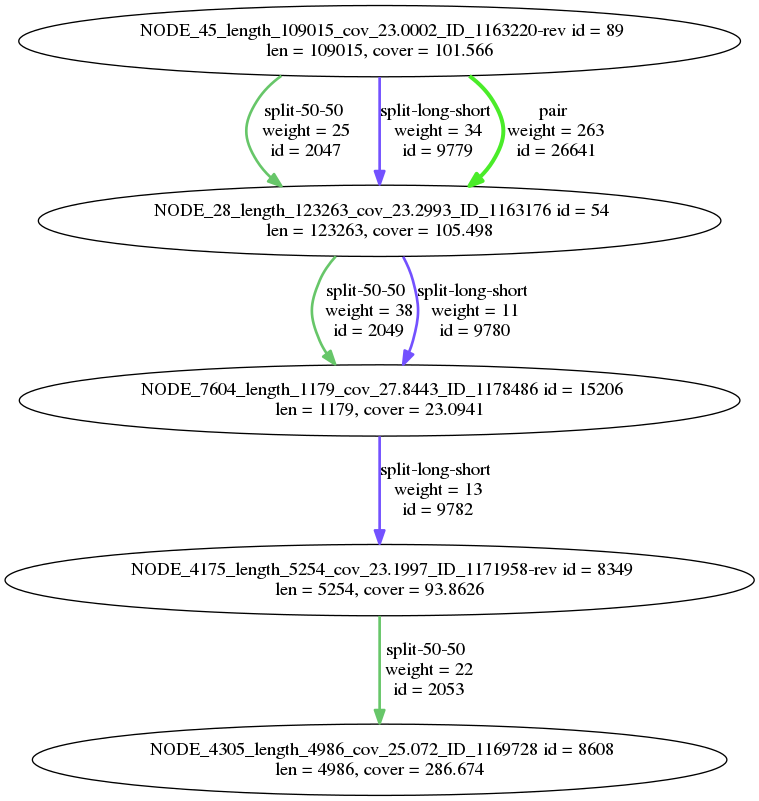
\includegraphics[width=0.35\linewidth]{celegExmp.png}
		\end{center}
	\end{itemize}
\end{frame}

\section{Использованные инструменты}
\begin{frame}[t]{Использованные инструменты}
%программа писалась не с нуля.
\begin{itemize}
	\item Язык разработки - \textbf{С++}
	\item \textbf{SeqAn} - библиотека для работы с 
	файлами в SAM/BAM и fasta/fastq форматах.  
	\item \textbf{gtest} - библиотека для тестирования.
	\item Программы для выранивания - \textbf{STAR, nucmer, bowtie2}. 
	\item \textbf{QUAST} - для анализа качетсва сборки. 
	\item \textbf{Tablet} - для визуализации выравненых ридов. 
\end{itemize}
\end{frame}

\section{Дальнейшие пути развития}
\begin{frame}[t]{Дальнейшее развитие}
\begin{itemize}
\item Разобраться в причинах текущих 
проблем с нахождением связей между 
контигами для данных A.thaliana.  

Тестирование программы на больших 
количествах данных. 

\cimg{athaliana.jpg}{0.20}
\item %Придумать методы решения данных проблем при построение графа. 
Новые методы нахождения связей и оценки их качества. 
\item Нахождение путей в графе и улучшение сборки. 
\end{itemize}
\end{frame}

\section{Спасибо за внимание}
\begin{frame}{Спасибо за внимание}
    \begin{center}
        Репозиторий: \\ \url{https://github.com/olga24912/bio_scaffolder}
    \end{center}
\end{frame}
\end{document}
